\documentclass[12pt]{article}

\usepackage{amsmath}
\usepackage{latexsym}
\usepackage{amstext}
\usepackage{array}
\usepackage{multirow}
\usepackage{graphicx}
\usepackage{caption}
\usepackage{subcaption}


%\usepackage{subcaption}

\pagestyle{plain}


\begin{document}
\title{Random loops -Supplementary material}

\begin{figure}[H]
 \begin{subfigure}[b]{0.3\textwidth}
 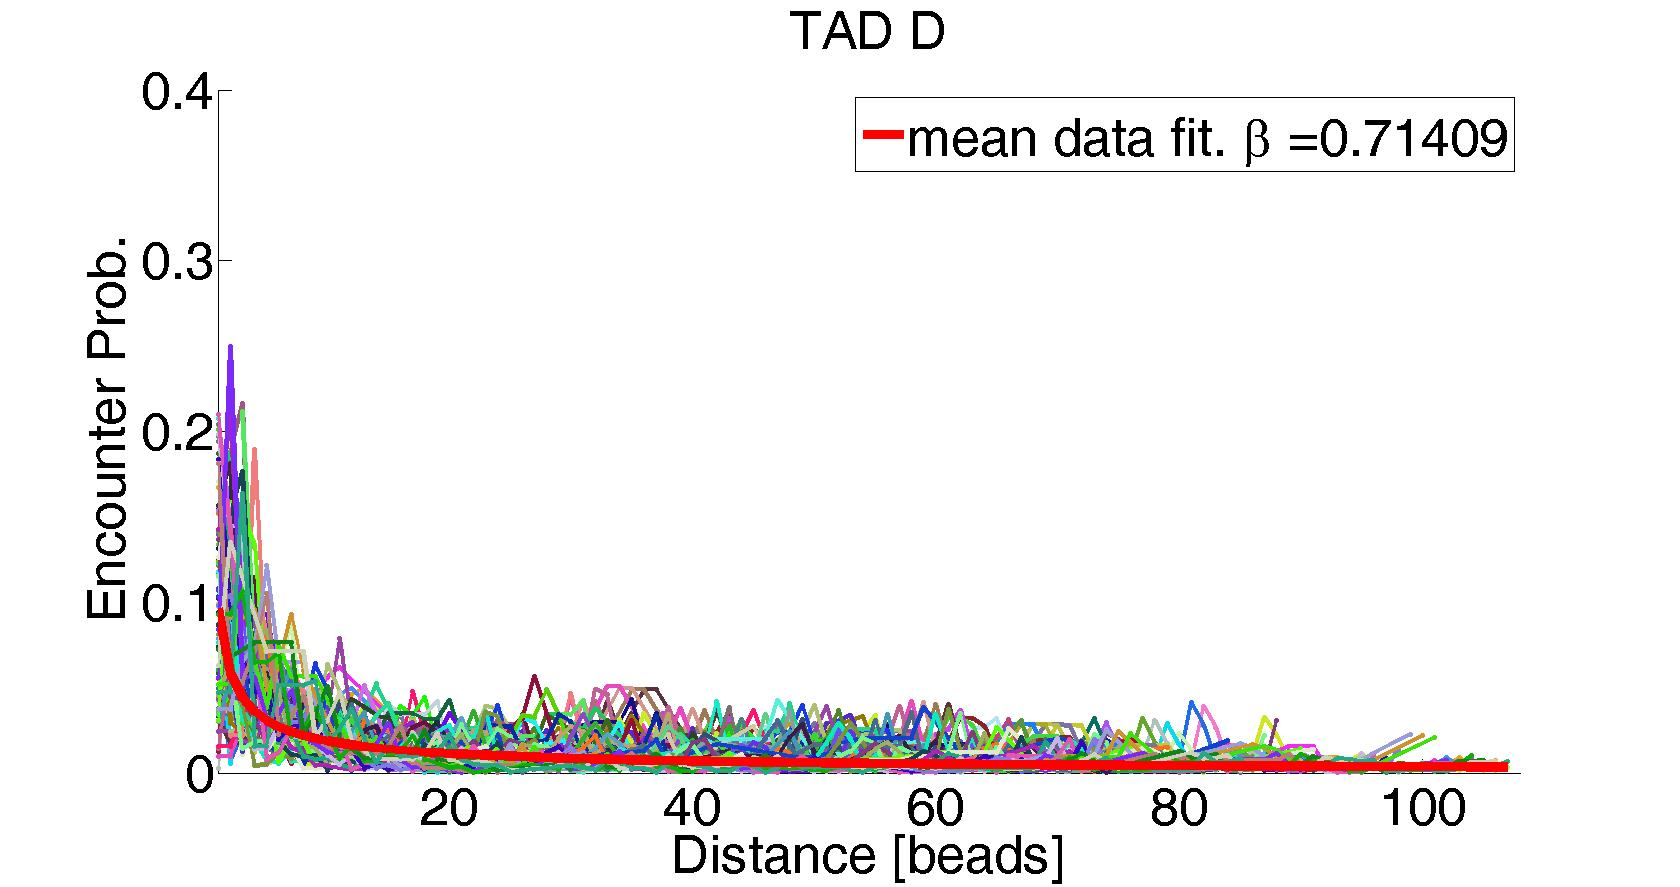
\includegraphics[scale=0.2]{meanDataFitTADD}
 \caption{}
 \end{subfigure}
 
 \begin{subfigure}[b]{0.3\textwidth}
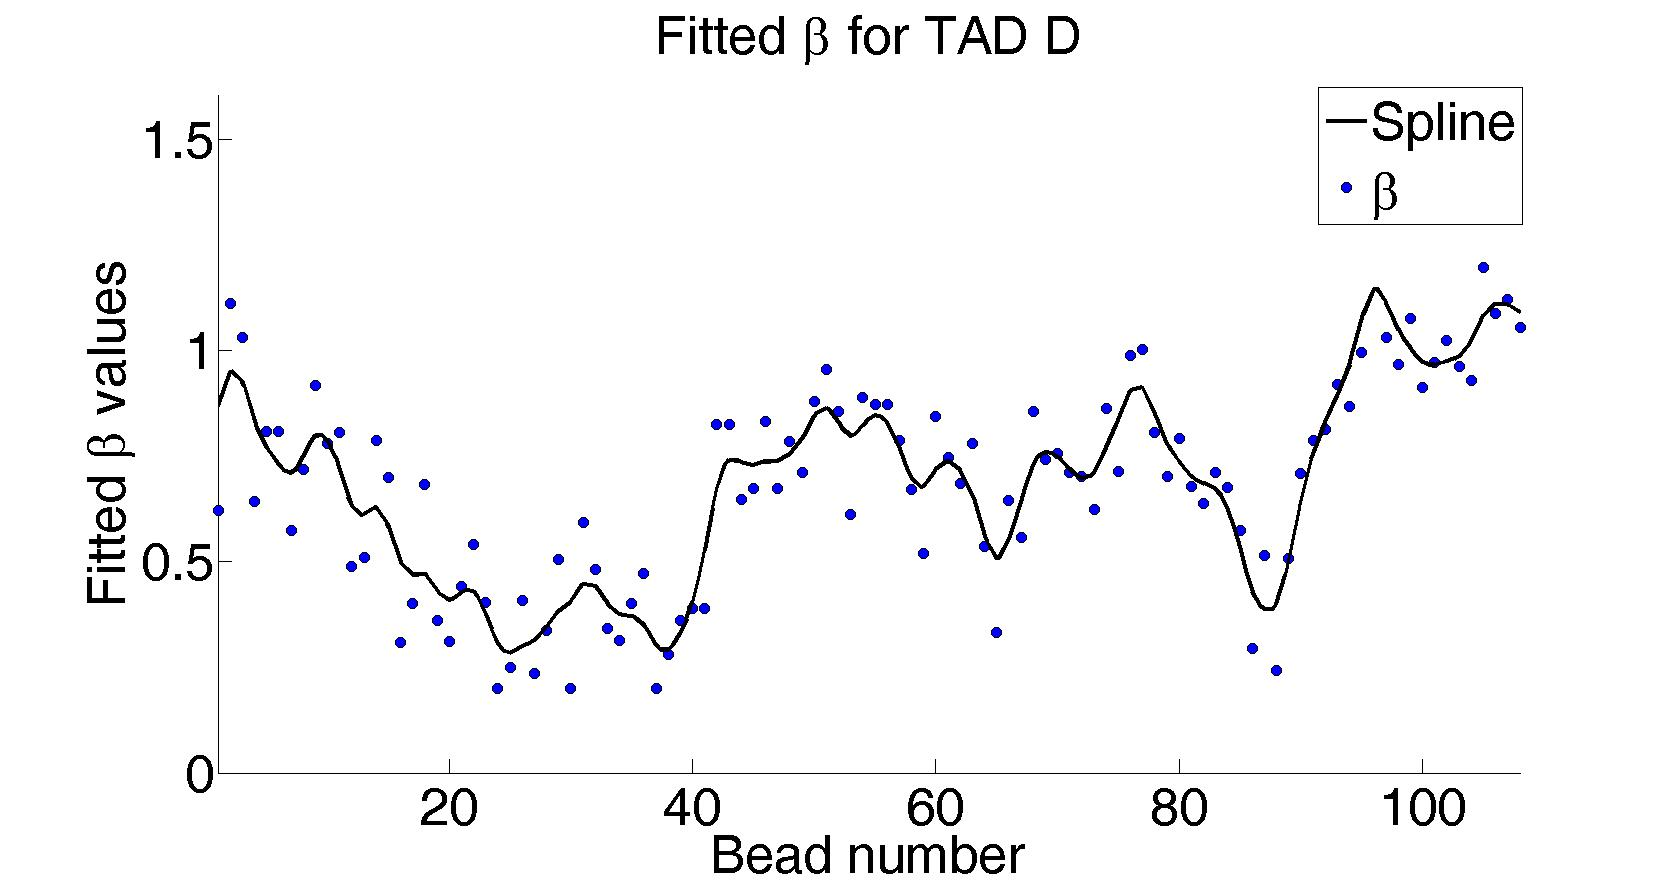
\includegraphics[scale=0.2]{fittedExpValuesWithSplineAverageTADD}
\caption{}
 \end{subfigure}
\caption{The encounter probability and the fitted $\beta$ values for TAD D.}
\end{figure}

\begin{figure}[H]
 \begin{subfigure}[b]{0.3\textwidth}
 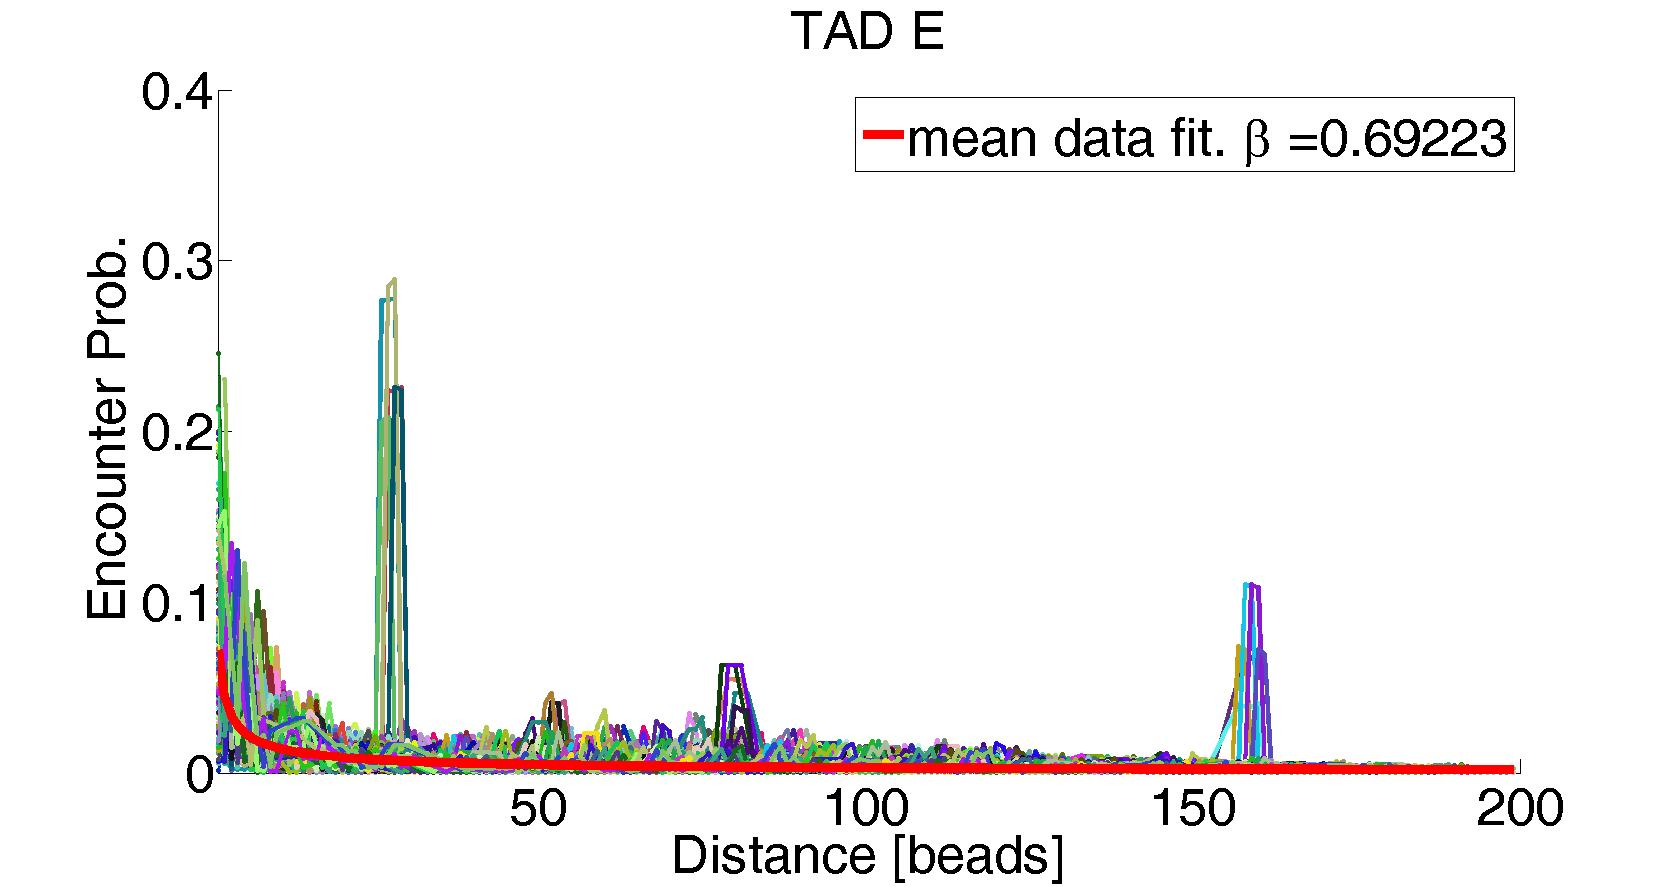
\includegraphics[scale=0.2]{meanDataFitTADE}
 \caption{}
 \end{subfigure}
 
 \begin{subfigure}[b]{0.3\textwidth}
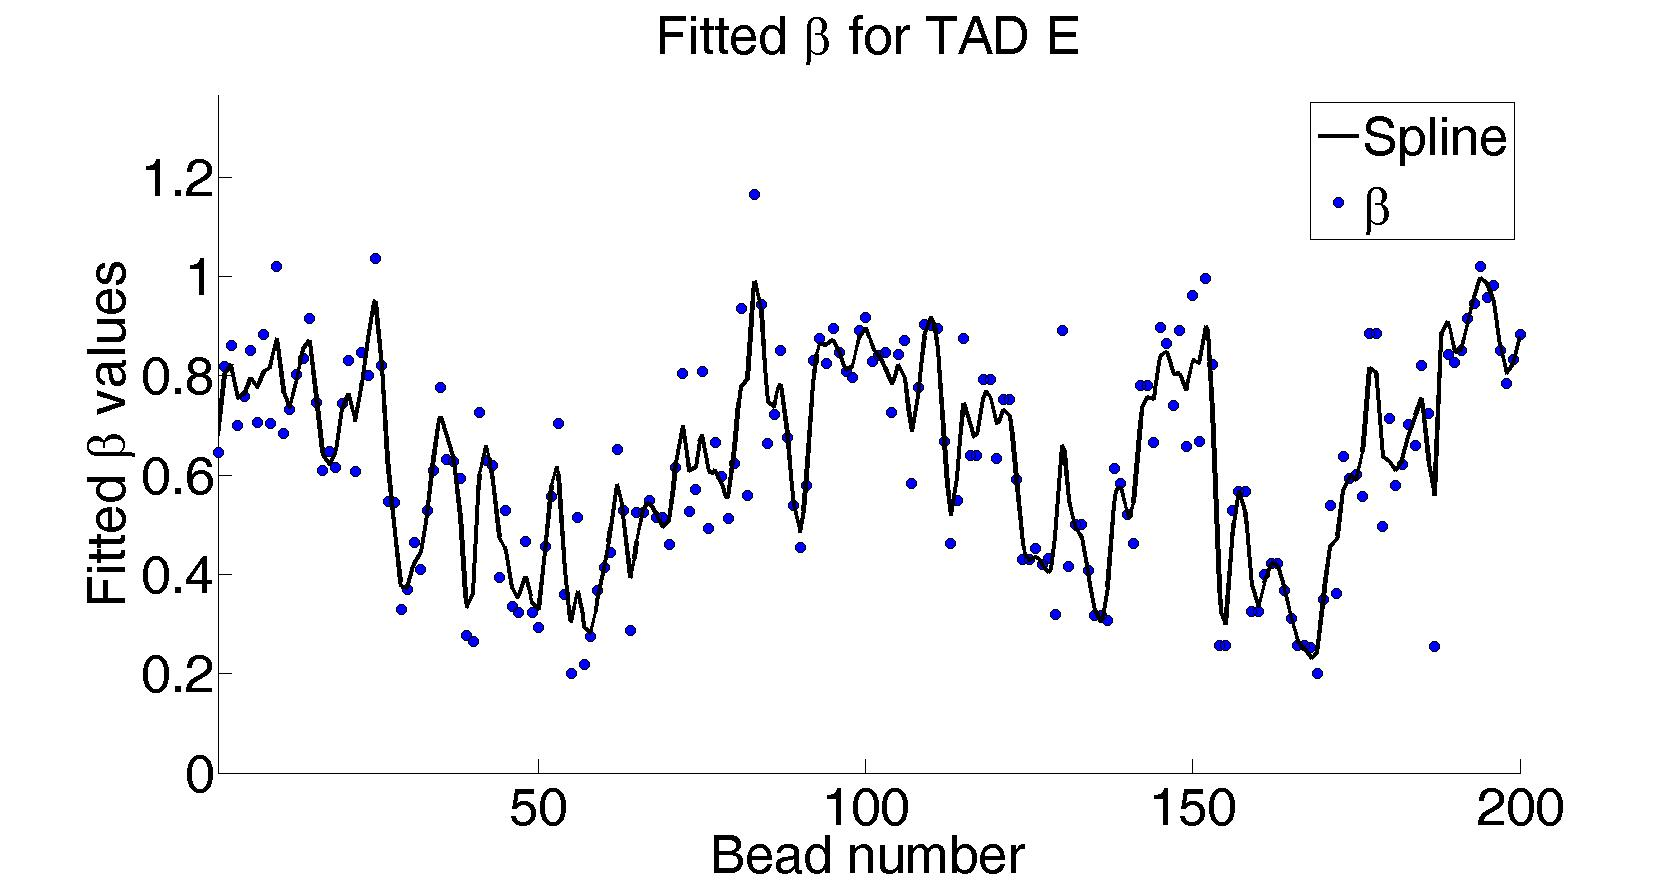
\includegraphics[scale=0.2]{fittedExpValuesWithSplineAverageTADE}
\caption{}
 \end{subfigure}
\caption{The encounter probability and the fitted $\beta$ values for TAD E.}
\end{figure}

\end{document}